\documentclass[a4paper,twoside,12pt,hidelinks]{article}

% Packages
% ---------------------

\usepackage{fancyhdr} % Head and foot options
\usepackage{hyperref} % Uses automatic references \autoref
\usepackage{titletoc} % Style table of contents with dots
\usepackage[T1]{fontenc}
\usepackage{libertine}
\usepackage{multirow}
\usepackage[libertine]{newtxmath} % Font
\usepackage[separate-uncertainty = true, multi-part-units=single]{siunitx} % Physical numbers and units
\usepackage{aas_macros} % To support Astronomy journal names in references
\usepackage{natbib}

% Page settings
% ---------------------

\usepackage[top=2cm, bottom=2.5cm,left=2.5cm,right=2.5cm]{geometry} %  Page margins
\setlength{\parskip}{\baselineskip} % Add space between paragraphs
\setlength{\intextsep}{20pt plus 2.0pt minus 2.0pt} % Add vertical space before and after tables and figures (http://tex.stackexchange.com/a/26522/101976)
\parindent=0cm % Remove the paragraph indent of the first line
\addtolength{\jot}{2\jot} % Double the line between equations
\def\arraystretch{1.5} % Increase the vertical table cell margin
\dottedcontents{part}[0em]{\bfseries}{0em}{1pc} % Use dots in the table of contents
\dottedcontents{section}[5em]{}{3em}{1pc} % Use dots in the table of contents
\renewcommand{\contentsname}{\centering Contents} % Center the table of contents header
\raggedbottom % Prevents spreading the page content vetically for non-full pages.
\setlength{\headheight}{20pt} % Height of the header

% Set vertical space around equations.
\AtBeginDocument{%
 \abovedisplayskip=15pt plus 5pt minus 5pt
 \abovedisplayshortskip=12pt plus 3pt
 \belowdisplayskip=15pt plus 5pt minus 5pt
 \belowdisplayshortskip=12pt plus 3pt minus 4pt
}

% Color the links and references
\hypersetup{
    colorlinks=true,
    linkcolor=blue,
    filecolor=magenta,
    urlcolor=blue,
    citecolor=blue
}

% Title page

\title{Photometric reduction of images of NGC 3201 stars and inference of their distance and age, and more\vspace{-1ex}}
\author{M. Funcich, E. Neumerzhitckii\vspace{-1ex}}
\date{\vspace{-5ex}}
\date{June 20, 2020}

\begin{document}

\setcounter{secnumdepth}{-1}
\renewcommand{\thepart}{}
\renewcommand{\thesection}{Part \Alph{section}}
\renewcommand{\thesubsection}{\Alph{section}.\arabic{subsection}}
\renewcommand{\partname}{}

\maketitle
\thispagestyle{empty} % Remove page number from title page
% \vspace{3.5cm} % Add space between the title and table of contents
% \pagebreak

% \tableofcontents
% \pagebreak


% Header and footer
% ---------------------

\pagestyle{fancy}
\fancyhf{}
\fancyhead[C]{Measuring the oscillations of a magnetometer's needle in magnetic field}
\fancyhead[LE,RO]{\thepage}


% Parts
% ---------------------


\begin{abstract}

\noindent Let me be clear. Change means a tax code that doesn't reward the lobbyists who wrote it, but the American workers and small businesses who deserve it. But privately, many Muslims recognize that Israel will not go away. No matter where it takes hold, government of the people and by the people sets a single standard for all who hold power: you must maintain your power through consent, not coercion; you must respect the rights of minorities, and participate with a spirit of tolerance and compromise; you must place the interests of your people and the legitimate workings of the political process above your party.
\end{abstract}

\vspace{1ex}% Additional space between abstract & rest of document

\section{Introduction}

\subsection{Thank you, and God bless America}

America! Tonight, if you feel the same energy that I do, if you feel the same urgency that I do, if you feel the same passion I do, if you feel the same hopefulness that I do - if we do what we must do, then I have no doubts that all across the country, from Florida to Oregon, from Washington to Maine, the people will rise up in November, and John Kerry will be sworn in as president, and John Edwards will be sworn in as vice president, and this country will reclaim its promise, and out of this long political darkness a brighter day will come. And throughout history, Islam has demonstrated through words and deeds the possibilities of religious tolerance and racial equality \citep{1992ASPC...23...68G}:

\begin{equation}
  \vec{E}(\vec{r}) = \frac{1}{4 \pi \epsilon_0} \int \rho(\vec{r}') \frac{\vec{r} - \vec{r}'}{|\vec{r} - \vec{r}'|^3} d\vec{r}'.
  \label{eq_q2_coulumbs_law_superposition}
\end{equation}


\subsection{A common dream, born of two continents.}

It's not enough, but it's helping \citep{2018A&A...616A...1G}. He's still speaking to our Catholic friends - who are holding up a consistent ethic of life that goes beyond abortion - one that includes a respect for life and dignity whether it's in Iraq, in poor neighborhoods, in African villages or even on death row. A lack of economic opportunity among black men, and the shame and frustration that came from not being able to provide for one's family, contributed to the erosion of black families - a problem that welfare policies for many years may have worsened (shown on \autoref{fig_barack_fishing}). This time we want to talk about the shuttered mills that once provided a decent life for men and women of every race, and the homes for sale that once belonged to Americans from every religion, every region, every walk of life. Of course, recognizing our common humanity is only the beginning of our task.

\begin{figure}[!ht]
  \centering
  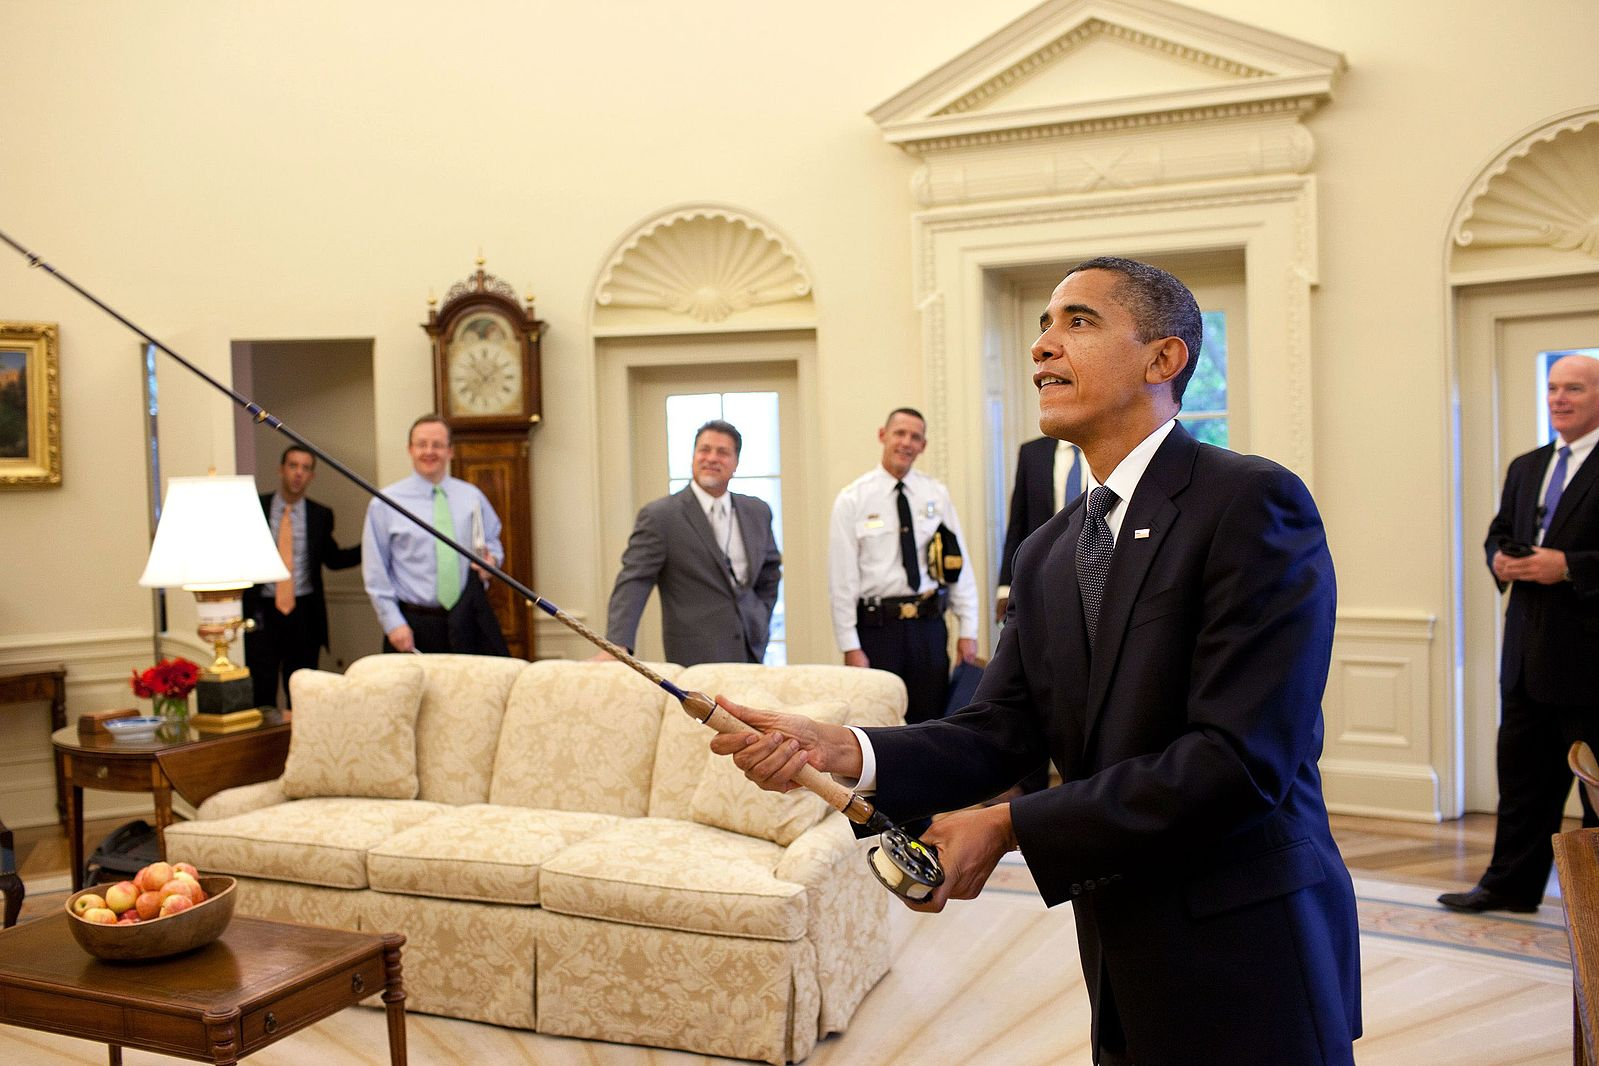
\includegraphics[width=0.7\textwidth]{images/President_Barack_Obama_tries_out_the_fly_fishing_rod_given_to_him_on_his_birthday_by_a_group_of_avid_fisherman_on_his_staff.jpg}
  \caption{President Barack Obama tries out the fly fishing rod given to him on his birthday by a group of avid fisherman on his staff, on Aug. 4, 2009.}
  \label{fig_barack_fishing}
\end{figure}

\section{Method} \label{sec_method}

\subsection{I wanted to be part of something larger}

For alongside our famous individualism, there's another ingredient in the American saga \citep{bessell2005standard}. I was too young to be involved in that movement, but I felt I could play a small part in the continuing battle for justice by helping rebuild some of Chicago's poorest neighborhoods. That is one option. In the face of that young student who sleeps just three hours before working the night shift, I think about my mom, who raised my sister and me on her own while she worked and earned her degree; who once turned to food stamps but was still able to send us to the best schools in the country with the help of student loans and scholarships. And while America in the past has focused on oil and gas in this part of the world, we now seek a broader engagement.

\subsection{We are one people}

In my first book, Dreams From My Father, I described the experience of my first service at Trinity: These challenges are not all of government's making. Over seven years ago, the United States pursued al Qaeda and the Taliban with broad international support.

\section{Results and analysis}

\subsection{That's not what I'm talking about}

It is not up in heaven \citep{1996ApJ...458..600B}. I am married to a black American who carries within her the blood of slaves and slaveowners - an inheritance we pass on to our two precious daughters. As William Faulkner once wrote, "The past isn't dead and buried. The men and women who gathered there could've heard many things. The situation in Afghanistan demonstrates America's goals, and our need to work together \autoref{tab_metallicities_literature}.

\begin{table*}
	\centering
	\caption{List of [Fe/H] abundances for NGC 288 available in the literature.}
	\label{tab_metallicities_literature}
	\begin{tabular}{lcc}
	\hline
	[Fe/H]	&	Source	&	Method\\
	\hline
	\hline
$-1.19 \pm 0.12$    & \cite{2014PASP..126..597H} & Spectroscopic study of 27 RGB stars	\\
$-1.39 \pm 0.01$	&	\cite{2000AJ....119..840S}	&	Spectroscopic study of 13 giant stars \\
$-1.24 \pm 0.04$	&	\cite{2000AJ....120.2569C}	&	Use 12 filters and Kurucz models \\
$-1.33 \pm 0.19$	&	\cite{1984AA...139...79N}	&	Photometric study \\
	\hline
	\end{tabular}
\end{table*}


\subsection{And nothing will change.}

I've seen it in the workers who would rather cut their hours back a day than see their friends lose their jobs, in the soldiers who re-enlist after losing a limb, in the good neighbors who take a stranger in when a hurricane strikes and the floodwaters rise \citep{refId0}. The situation in Afghanistan demonstrates America's goals, and our need to work together.

\section{Discussion} \label{sec_discussion}

He was a good-looking kid, six two, six three, clear eyed, with an easy smile. More of you have lost your homes and even more are watching your home values plummet. And when one of his chief advisors - the man who wrote his economic plan - was talking about the anxiety Americans are feeling, he said that we were just suffering from a "mental recession," and that we've become, and I quote, "a nation of whiners." This tolerance is essential for religion to thrive, but it is being challenged in many different ways.

To the Joshua generation, these challenges seem momentous - and they are. That promise is our greatest inheritance. There is also one rule that lies at the heart of every religion - that we do unto others as we would have them do unto us. This truth transcends nations and peoples - a belief that isn't new; that isn't black or white or brown; that isn't Christian, or Muslim or Jew.

\section{Conclusion}

But at the end of the day, we cannot walk away - not for the sake of passing a bill, but so that we can finally address the real concerns of Americans and the persistent hopes of all those brothers and sisters who want nothing more than their own chance at our common dream. And you know what - it's worked before.

What we have already achieved gives us hope - the audacity to hope - for what we can and must achieve tomorrow. I would not be running for President if I didn't believe with all my heart that this is what the vast majority of Americans want for this country. But it is where we start. And when innocents in Bosnia and Darfur are slaughtered, that is a stain on our collective conscience.



% Bibliography
% ---------------------

\bibliographystyle{apalike}
\bibliography{assignment}

\end{document}
